% THIS IS AN EXAMPLE DOCUMENT FOR VLDB 2012
% based on ACM SIGPROC-SP.TEX VERSION 2.7
% Modified by  Gerald Weber <gerald@cs.auckland.ac.nz>
% Removed the requirement to include *bbl file in here. (AhmetSacan, Sep2012)
% Fixed the equation on page 3 to prevent line overflow. (AhmetSacan, Sep2012)

\documentclass{vldb}
\usepackage{graphicx}
\usepackage{balance}  % for  \balance command ON LAST PAGE  (only there!)



\begin{abstract}
  Despite the growing popularity of techniques related to graph summarization, a general operator for the flexible nesting of graphs is still missing.
  We propose a novel nested graph data model and a powerful graph nesting operator. In contrast to existing approaches, our approach is able to summarize vertices and paths among vertex groups within a single query. Further on, our model supports partial nestings under the preservation of original graph elements as well as the full recovery of the original graph. We propose an efficient nesting algorithm (THoSP) that is able to perform vertex and path nestings in a single visit of the input graph. Results of an experimental evaluation show that THoSP outperforms equivalent implementations based on graph (Cypher, SPARQL), relational (SQL) and document oriented (ArangoDB) databases.
\end{abstract}

\begin{document}
\fancyhead{}
\title{THoSP: an Algorithm for Nesting Property Graphs}
%\numberofauthors{3} 
%\renewcommand{\auwidth}{0.23\linewidth}
%\author{
%\alignauthor
%Giacomo Bergami\\
%       \affaddr{University of Bologna}\\
%       \affaddr{CSE Department}\\
%       \affaddr{Bologna, Italy}\\
%       \email{giacomo.bergami2@\\
%       	unibo.it}
%% 2nd. author
% \alignauthor
%André Petermann\\
%       \affaddr{University of Leipzig}\\
%       \affaddr{Leipzig, Germany}\\
%       \email{petermann@informatik.\\
%       	uni-leipzig.de}
%% 3rd. author
%\alignauthor Danilo Montesi\\
%       \affaddr{University of Bologna}\\
%       \affaddr{CSE Department}\\
%       \affaddr{Bologna, Italy}\\
%       \email{danilo.montesi@\\
%       	unibo.it}
%}


%\renewcommand{\shortauthors}{[Authors]}

\author{Giacomo Bergami}
\affiliation{\institution{University of Bologna}}
\email{giacomo.bergami2@unibo.it}

\author{André Petermann}
\affiliation{\institution{University of Leipzig}}
\email{petermann@informatik.uni-leipzig.de}

\author{Danilo Montesi}
\affiliation{\institution{University of Bologna}}
\email{danilo.montesi@unibo.it}


\begin{CCSXML}
	<ccs2012>
	<concept>
	<concept_id>10002951.10002952.10002953.10010146</concept_id>
	<concept_desc>Information systems~Graph-based database models</concept_desc>
	<concept_significance>300</concept_significance>
	</concept>
	<concept>
	<concept_id>10002951.10002952.10003190.10003192.10003210</concept_id>
	<concept_desc>Information systems~Query optimization</concept_desc>
	<concept_significance>300</concept_significance>
	</concept>
	</ccs2012>
\end{CCSXML}

\ccsdesc[300]{Information systems~Query optimization}
\ccsdesc[300]{Information systems~Graph-based database models}

\keywords{Graph Nesting, Nested graphs, Nested Property Graphs}

%
%\author{G.K.M. Tobin}
%\authornote{The secretary disavows any knowledge of this author's actions.}
%\affiliation{%
%	\institution{Institute for Clarity in Documentation}
%	\streetaddress{P.O. Box 1212}
%	\city{Dublin}
%	\state{Ohio}
%	\postcode{43017-6221}
%}
%\email{webmaster@marysville-ohio.com}
%
%\author{Lars Th{\o}rv{\"a}ld}
%\authornote{This author is the
%	one who did all the really hard work.}
%\affiliation{%
%	\institution{The Th{\o}rv{\"a}ld Group}
%	\streetaddress{1 Th{\o}rv{\"a}ld Circle}
%	\city{Hekla}
%	\country{Iceland}}
%\email{larst@affiliation.org}
%
%\author{Valerie B\'eranger}
%\affiliation{%
%	\institution{Inria Paris-Rocquencourt}
%	\city{Rocquencourt}
%	\country{France}
%}
%\author{Aparna Patel}
%\affiliation{%
%	\institution{Rajiv Gandhi University}
%	\streetaddress{Rono-Hills}
%	\city{Doimukh}
%	\state{Arunachal Pradesh}
%	\country{India}}
%\author{Huifen Chan}
%\affiliation{%
%	\institution{Tsinghua University}
%	\streetaddress{30 Shuangqing Rd}
%	\city{Haidian Qu}
%	\state{Beijing Shi}
%	\country{China}
%}
%
%\author{Charles Palmer}
%\affiliation{%
%	\institution{Palmer Research Laboratories}
%	\streetaddress{8600 Datapoint Drive}
%	\city{San Antonio}
%	\state{Texas}
%	\postcode{78229}}
%\email{cpalmer@prl.com}
%
%\author{John Smith}
%\affiliation{\institution{The Th{\o}rv{\"a}ld Group}}
%\email{jsmith@affiliation.org}
%
%\author{Julius P.~Kumquat}
%\affiliation{\institution{The Kumquat Consortium}}
%\email{jpkumquat@consortium.net}

\fancyhead{}
\maketitle



% !TeX root = 00_nesting_paper-Wall-Pedantic.tex

\section{Introduction}
Graphs allow flexible analyses of relationships among data objects. Thus, graph data management systems play an increasing role in present data analytics. Graphs have been already used as a fundamental data structure to represent data within different contexts such as corporate data \cite{success,Park2016355}, social networks \cite{xie,BrodkaK14} and linked data \cite{Vasilyeva13}.
Despite an increasing number of applications, a general operator that aggregates a single graph in a roll-up fashion is still missing. %partitions which the aforementioned vertices represent.
 The operation of adding structural aggregations to an existing graph is called \textit{graph nesting}.
A respective operator shall not only create a new graph of \textit{nested vertices} and \textit{nested edges}, each containing subgraphs of the original input graph, but also preserve the vertices and edges that are not affected by the actual operation. Further on, the operator must ensure that the nested elements can be freely unnested such that the original graph may be obtained back again. Vertices or edges of the original graph will be called \textit{members} of a nested vertex or edge, if they appear in its underlying subgraph.

\begin{figure}[!t]
  \begin{minipage}[!t]{0.5\textwidth}
    \centering
    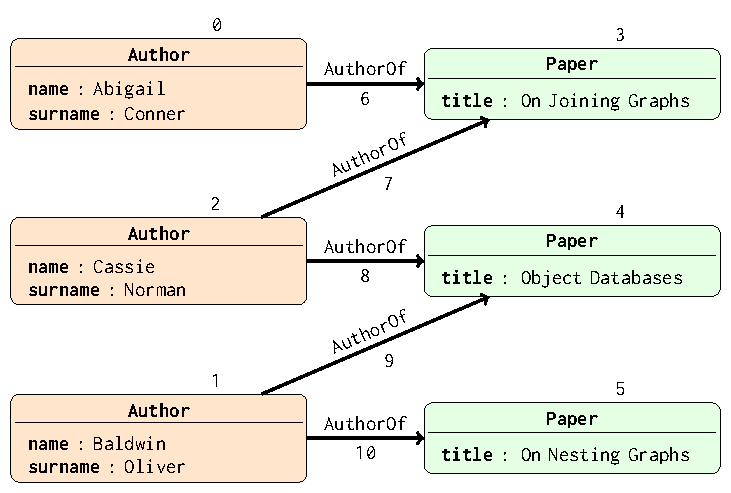
\includegraphics[width=.8\textwidth]{images/nesting/patterns/04bibliography.pdf}
    \subcaption{Input bibliographical network.}
    \label{fig:inputbibex2}
  \end{minipage}
  \medskip

  \begin{minipage}[!t]{0.5\textwidth}
    \centering
    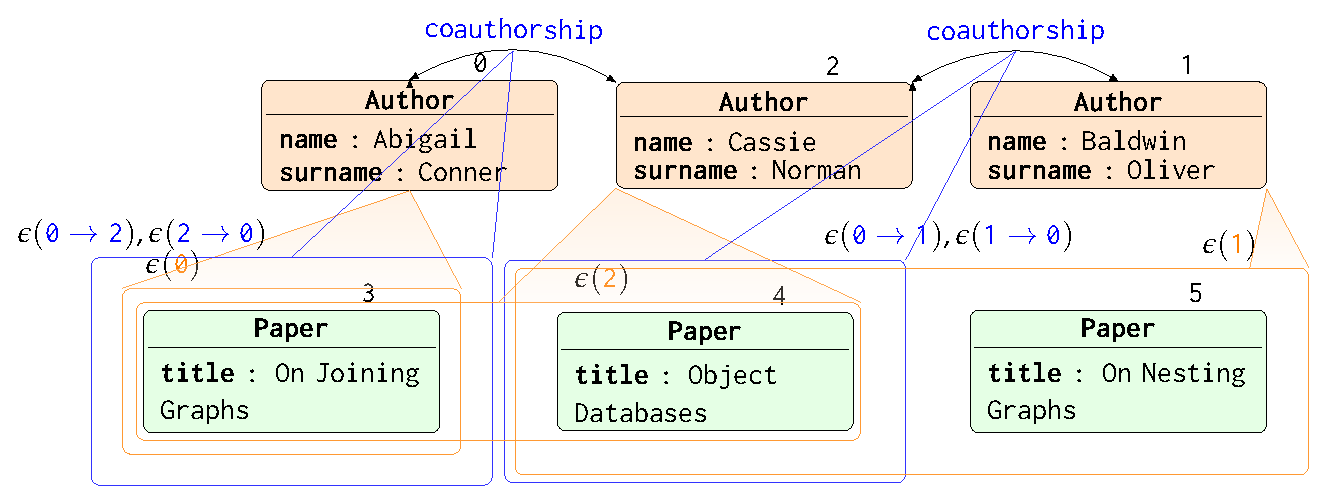
\includegraphics[width=\textwidth]{images/nesting/patterns/042nested.pdf}
    \subcaption{Nested result: given two \texttt{Author}s $\color{orange}a$ and $\color{orange}a'$, there exist two  \texttt{coauthorship} edges, $\color{blue}a\to a'$ and $\color{blue}a'\to a$ if and only if they share some authored paper contained respectively in $\epsilon({\color{blue}a\to a'})$ and $\epsilon({\color{blue}a'\to a})$. Moreover, each author $\color{orange}a$ is associated to the set of his authored papers $\epsilon({\color{orange}a})$. }
    \label{fig:outputnested}
  \end{minipage}
\caption{Nesting a bibliographic network: the provenance information is nested within the original node. }
\label{fig:bibex2}
\end{figure}

\begin{ex}[label=ex1]
Figure \ref{fig:inputbibex2} represents a bibliographic network with (at least) \textsc{Author}s and \textsc{Paper}s as vertices and \textsc{authorOf} relationships as edges which connect authors to papers they have authored. With the graph nesting operator, we want to ``roll up'' the network into a coauthorship network (Figure \ref{fig:outputnested}). Here each \textsc{Author} will be connected by a \textsc{coAuthor} edge with another \textsc{Author}(2) if they have published at least one paper in common.
More precisely, each resulting \textsc{Author}(2) vertex shall contain authored papers as vertices and each \textsc{coAuthor} edge all coauthored papers with regard to source and target \textsc{Author}s. However, we want to exclude \textsc{coAuthor} hooks over the same vertex.
\end{ex}

In a resulting nested graph, edges connecting nested vertices express that members of the nested vertices are connected by an edge or, more generally, by a path in the original graph.
In contrast to this general approach, current literature distinguishes between \textit{vertex summarization} and \textit{path summarization}. Thus, it is not possible to define a single algorithm that evaluates both kinds of patterns at the same time. Before outlining our proposed algorithmic solution, let's have a look on these existing approaches:

The \textit{vertex summarization} strategies group vertices in the manner of the relational \texttt{GROUP BY} operation and aggregate edges accordingly \cite{JunghannsPR17}. In this class of operations summarized edges can only be formed by edges that directly connect members of summarized vertices in the original graph. In other words, these approaches cannot freely nest edges, for example, it is not possible to aggregate paths. Since most of vertex summarization techniques are based on graph partitioning, they further provide no support for nested vertices and edges with overlapping members \cite{yin,Tian20085,jakawat}.
Exceptions are HEIDS \cite{ChengJQ16} and Graph Cube \cite{Zhao11}, which perform graph summarizations of one single graph over a collection of non pairwise disjoint subgraphs. However, the union of these underlying subgraphs must be equivalent to the original graph, i.e., it is not possible to take vertices and edges of the original graph over to the summarized graph or to represent outliers that belong to no group.

%To overcome to this graph operation limitation, this thesis proposes the \textbf{graph nesting} operator, thus providing a general graph summarization technique.
%A straightforward implementation  proves to be inefficient, because the visit of such graph collections of size $k$ (to be nested within the graph operand) implies to perform, in the worst case scenario, $|g|^k$ visits of the graph operand $g$: this results into an exponential algorithm, because the size of $k$ may vary, while $|g|$ is fixed. This implies that the graph must be always visited more than once, even if this may not be required. Even though this general operator proves to be inefficient in practice, it allows to detect a broader class of problems and of optimizable algorithms.
%In order to reduce the graph visiting cost from $|g|^k$ to $O(|g|)$, we could use a graph traversal approach: instead of pre-computing $k$ subgraphs of $g$ that are going to be later on used to nest $g$, we can directly perform the graph nesting while visiting the graph, thus allowing  not to perform additional costs for comparing the resulting graphs in a later step. The following example shows how such queries can be efficiently formulated and implemented.
By contrast, \textit{path summarization} techniques allow the aggregation of multiple paths among pairs of source and target vertices that share the same properties.
%At the time of the writing, such approaches can be performed only over (graph) query languages.
Currently, approaches to path summarization can only be found within graph query languages.
%The problem with both path and vertex summarizations is that no general class of either source and target vertices can be used as an outcome of a previous community detection \cite{xie,berlingerio11} or data cleaning and alignment phase \cite{ALIEH17} without rewriting the previously extracted data into an explicit query, thus requiring an additional pre-processing step and thus making such approach not as flexible as required by data integration scenarios. %%initial query each time after different vertex data is extracted, thus not allowing to use such query definition for general data integration scenarios.
%This problem is also reflected by 
These languages also support vertex summarization, but no combination of both approaches in a single step.
%This constraint thwarts the advantages of performing vertex and path summarizations concurrently:
Cypher, the query language of the productive graph database Neo4j, can perform distinct aggregations only within distinct \texttt{MATCH} clauses. SPARQL, the standard query language of the resource description framework (RDF), requires to combine vertex and path aggregation with a \texttt{UNION} operator, i.e., the same input graph must be visited twice.
%As a result, the query plan optimizers of such query languages do not allow to avoid to visit one same graph more than once whether possible.

This paper shows that such query language limitations can be reduced by using a graph nesting operator, which performs both vertex and path summarization queries concurrently with only a single visit of the input graph. %The following example provides an example of how such query can be formulated and performed. --> Old example
We propose graph patterns to declare graph nesting operations and propose algorithmic optimizations as well as a specific physical model for efficient execution.
	
\begin{figure}[!t]
	\centering
	\begin{minipage}[!t]{0.5\textwidth}
		\centering
		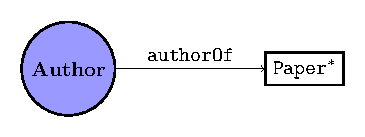
\includegraphics[width=.6\textwidth]{images/nesting/patterns/00_vertex_pattern.pdf}
		\subcaption{Vertex summarization pattern ($V$). Author is the vertex grouping reference $\gamma_V$.}
		\label{fig:vertexPat}
	\end{minipage} \begin{minipage}[!t]{0.4\textwidth}
		\centering
		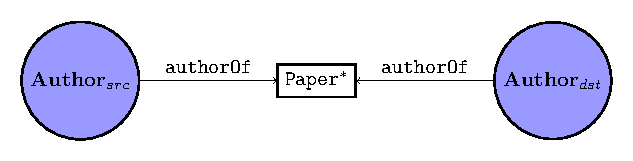
\includegraphics[width=1\textwidth]{images/nesting/patterns/00_path_pattern.pdf}
		\subcaption{Path summarization pattern ($E$). Author$_{src}$ and Author$_{dst}$ are respectively edge grouping references $\gamma_E^{src}$ and $\gamma_E^{dst}$.}
		\label{fig:pathPat}
	\end{minipage}
  \caption{Vertex and Path summarization patterns for the query expressed in the running example. Vertex and edge grouping references are marked by a light blue circled node. As we can see, the vertex grouping reference depicts the same property expressed by edge grouping references.}
\label{fig:patterns}
\end{figure}


\begin{ex}[label=ex2,continues=ex1]
	Figure \ref{fig:patterns} shows summarization patterns to describe the vertex ($g_V$) and path ($g_E$) nestings of our bibliographic network example: the former will create a nested \textsc{Author}(2) vertex and the latter will create a \textsc{coAuthor} nested edge. Given that $g_V$ appears twice in $g_E$, we may also pre-istantiate the pattern $g_V$ by visiting $g_E$ once. The two patterns have different key roles: while the vertex summarization retrieves all the papers that one author has published and nest them within one single matched author, the path summarizations return all the papers authored by two different authors and creates an edge between the two previously nested vertices. %This construction implies that a join between the two paths must be carried out.
	For each vertex pattern we're going to elect one vertex as a \textbf{vertex grouping reference} ($\gamma_V$), in which we're going to nest the matched vertices and edges  during the graph traversal. Similarly, each edge path summarization pattern is going to elect a source ($\gamma_E^{src}$) and a target ($\gamma_E^{dst}$) vertex, which are going to be called \textbf{edge grouping references}: such vertces must both coincide with the vertex grouping references, so that the newly generated edge will have as sources and target the previously vertex-nested elements. In particular, this paper focuses on $g_E$ where $\gamma_E^{src}$  and $\gamma_E^{dst}$ are separated by a two-edge (hop) distance.
	
	
	We solve this problem by visiting the graph only once: %by visiting the graph starting from the vertices:
	If the current vertex is a \textsc{Paper}, traverse backwards all the \textsc{authorOf} edges, thus reaching all of its \textsc{Author}s ($\gamma_E^{src}$ and $\gamma_E^{dst}$), that are going to be \textsc{coAuthor}s for at least the current paper. Instead of associating the nesting content at the end of the graph visiting process, I can incrementally define the subgraph to be nested by using a separated nesting index: by visiting the two distinct \textsc{Author} vertices adjacent to the current \textsc{Paper}, the latter one shall be contained in both final \textsc{Author}(2) vertices, thus allowing the definition of a  \textsc{coAuthor} edge. %%The remaining types of vertices and edges %All the other vertices and edges
	%%may be discarded. %as a starting point for the graph visiting process
	By doing this, only the edges are visited twice, but the vertices are visited only once. These patterns allow to reach the optimal solution.
	
	%This pattern comparison remarks that, in order to reduce the graph time visit, we must start from visiting the \texttt{Paper}, which is shared among the two distinct patterns, and then keep going with the graph visit by exploring the source and target vertices. 
\end{ex}

%There might be other possible patterns that can be optimized, but we're going to focus just on vertex and path summarization patterns where edge grouping references are connected to each other at a 2 edge step distance (Section \ref{sec:THOSPA}). We're also going to show how such optimizations can be detected beforehand by looking at the pattern representation.


In the remainder of this paper, we will show that our algorithmic approaches reduce the time complexity of the visiting and nesting problem. Further on, our optimized data structure requires less indexing time than our competitors. This is achieved by the following contributions:

\begin{itemize}
	\item We propose a \textbf{Nested Graph Data Model} that is capable to implement the aforementioned solution of our example scenario. We use an optimized physical model that differs from the logical one (Section \ref{sec:model}).

	\item We provide  a general definition of a \textbf{Graph Nesting Operator} which combines vertex and path summarization approaches to nesting graphs (Section \ref{sec:nestingdef}).
	\item We introduce the  \textbf{\textsc{{Two HOp Separated Patterns}} (THoSP)} algorithm for graph nesting (Section \ref{sec:THOSPA}). We present the results of an experimental evaluation that compare it to alternative implementations using graph (SPARQL, Cypher), relational (SQL) and document oriented (AQL) query languages: our solution outperforms all competitors by at least one order of magnitude with regard to the sum of both indexing and query evaluation time (Section \ref{sec:nestexpeval}).

%  the aforementioned solutions evaluated on such databases with their respective query languages . Consequently, our data model also proved to be crucial in providing an enhanced implementation of the specific graph nesting task.
	%\item A general strategy on how to extend the THoSP algorithm for patterns having vertex and edge grouping references is provided (Section \ref{sec:optimizableClass}).
	%%\item By extending the concept of binary predicates into edges, Edge Joins are introduced as a preliminary step towards the definition of Graph Nesting (Chapter \ref{cha:nesting}).
\end{itemize}

The source code for THoSP is provided at \texttt{\color{red}[Link removed for double-blind review]}.

% !TeX root = 00_paper_entrypoint.tex
\section{Related Work}

\subsection{Nested Graph Representations}
\textbf{Statecharts} \cite{statecharts} represent one of the first applications of nested graphs for complex systems modelling. This choice allowed the representation of multiple abstraction levels at the same time: each node represents a  state or ``configuration'' of the system, and each edge represents a transaction between two different states on a given event. In order to represent different nesting levels, each node may contain other states and edges. As a consequence,  there is no distinction between (simple) states and states containing other states. Given that this model was not designed for data representations, vertices and edges are labelled but cannot contain any property-value association. 
This model allows both \textit{external edges} and \textit{internal edges}: an edge  $e$ will be called \textit{external} if its source (or target) is contained by the target (or source) but neither of them contains $e$; the edge will be called \textit{internal} when the containing vertex (either its source or target) also contains the edge. Besides of state representation purposes, this model has also been  used for both modelling the evolution of \textit{pathophysiological} states and to describe the clinical treatments to which the patient must undergo. This model also allowed to subdivide each treatment  into smaller and consequential procedures \cite{NestedGlaucoma}.

Statecharts were also adopted as a basis for the subsequent \textbf{hypernode} data model \cite{Poulovassilis1994}. Unlike statecharts, hypernodes allow neither edge labelling nor external and internal edges. As previously stated for statecharts, even this model does not allow to fully represent a property graph, since the attribute-value association must be necessarily expressed as a relation between two different vertices.  A first extension of the hypernode model towards data representation is represented by CoGITaNT \cite{GenestS98}, where any type of edge (thus including internal and external ones) are included and data is firstly contained inside a node. Nested graphs are also supported by GraphML \cite{graphml} and GXL \cite{GXL}.

Current literature uses two different approaches for extending
% Two different approaches have been used to extend 
graph databases to support nesting operations:
some try to overcome graph data structure limitations by extending their query languages, while others try to extend the data structures used for both input and intermediate computations. Among the first type of approaches, \cite{Etcheverry2012} proposes the definition of a RDF  vocabulary over which the OLAP  cube can be defined. On top of this ``structured'' RDF graph, an algorithm generates the SPARQL query that will allow to perform either the roll-up or the drill-down operation. This implies that each possible computation over the data view has to be always recomputed on top of the raw data as in ROLAP systems, thus thwarting the benefits of updating the intermediate query result. On the other hand, the last type of approaches has been recently widely investigated  and seems to be more promising with regard to optimization techniques. In these approaches \cite{Tian20085,ChenYZHY08,Qu2011}, graph data structures are associated with external graph indices and, thus, allow to connect one graph to a broader one with respect to the roll-up query. As a consequence, these solutions do not allow to freely expand any aggregate components at the same time but can only backtrack the aggregation to a previous known state. %Some further details are going to be provided on Chapter \vref{cha:nesting}, where such operator will be implemented on a specific algorithm.
%As it will be showed in Chapter \ref{cha:graphsdef}, in order to meet such goals the nesting indices are going to be directly embedded within the definition of the nested (graph) data model, thus allowing to extend all the aforementioned approaches.


\subsection{Databases and Query Languages}\label{subsec:pathsumm}
As previously mentioned, some recent  query languages support graph nesting semantics by exploiting the underlying data model's features. To express the query presented in our running example, these query languages must support id collections or nested representations.
For these reasons, we firstly select PostgreSQL which, by extending the SQL-3 syntax and by allowing JSON data, provides an \texttt{array\_agg} aggregation function. The latter collects (i.e., groups) the result-set into arrays.  We  represent  graphs by  storing edge triples in the following form:
\begin{center}
 \texttt{Edge}(\textit{edgeId},\;\textit{sourceId},\;\textit{edgeLabel},\;\textit{targetId})
\end{center}
In our running example, nested vertices  are obtained by 
grouping edges by \textit{sourceId} and collecting all target's id results via \texttt{array\_agg}. Similarly, our nested edges are obtained by joining consecutive \texttt{Edge}s and then grouping  by  distinct \textit{sourceId} and \textit{targetId}  vertices limiting the two hop path; the list of all the \textsc{Paper}s is collected via \texttt{array\_agg}. The overall graph nesting cannot be created in one single SQL query, because we cannot distinctively group the same dataset in different ways. Instead, we must perform two distinct aggregations (see Listing \ref{SQLNesting} in Appendix).


Despite the fact that SPARQL  may represent the graph nesting query as a single statement, a \texttt{UNION} clause implies a separate visit for the two graph patterns. The first pattern presented in Listing \ref{SPARQLNesting} (see Appendix) allows to traverse those  patterns matching the coauthorship statement in Figure \ref{fig:pathPat}, so that they can be nested within the created \textsc{CoAuthorship} edge. The second part returns the remaining \textsc{Paper} associations that have been authored by one single \textsc{Author}. In the first case, the edge nesting is performed via the association of different \texttt{<http://cnt.io/nesting>} properties departing from one single  \textsc{coAuthorship} edge (\texttt{?newedge}).

ArangoDB is a document-oriented NoSQL database, which query language AQL allows the access and the creation of nested members. An example of how such graph nesting query can be carried out in AQL is presented in Listing \ref{AQLQueryNesting}: in this scenario we assume that we've previously loaded our graph data with the default ArangoDB format, where  vertices are indexed by id while edges are also indexed by source and target vertex id. Even though AQL returns JSON documents instead of relational tables, we can state that its resulting query plan is similar to PostgreSQL's query plan.
%
%Let us consider the following query that will be express in our different languages:
%``\textit{Total number of orders handled by each employee. Only list employees that handled more than 100 orders}''
%
%At this point we immediately notice that NautiLOD and G could not express the summarization since those languages
%are graph traversal languages for pattern matching: consequently they could only select paths and subgraphs but
%they do not aggregate (summarize) nodes. In this case a bag of both employees and the number of the orders
%is returned. Since the result is a bag of values, we cannot obtain a graph as an output, and hence we cannot establish some new edges through the employee and the aggregated value of the sales.
%
%\begin{lstlisting}[caption={Summarization query in Gremlin},language=gremlin,frameround=fttt,frame=trBL]
%graph = TinkerGraph.open()
%graph.io(IoCore.gryo()).readGraph('/path/to/graph')
%g = graph.traversal()
%
%g.V().hasLabel("Employee").match(
%      __.as("emp").in("SalesEmployee").hasLabel("Sales").count()
%                                      .as("ordersByEmployee"),
%      __.as("ordersByEmployee").is(gt(100))
%).select("emp", "ordersByEmployee")
%\end{lstlisting}
%\medskip
%
%The SPARQL query returns a table with two attributes, where the first is the Employee ID and the
%second element is the number of its handled orders. In this case the output is expressed as a table.
%
%\begin{lstlisting}[caption={Summarization query in SPARQL: Table},language=sparql,frameround=fttt,frame=trBL]
%PREFIX ex:<http://example.it/Relations#>
%
%SELECT	 ?emp, (COUNT (?sales) AS ?ordersByEmployee)
%WHERE    {
%          ?sales a                 ex:Sales;
%                 ex:SalesEmployee  ?emp.
%          ?emp   a                 ex:Employee.    
%         }
%GROUP BY ?emp
%HAVING   COUNT(?orderNo) > 100
%\end{lstlisting}
%
%With the \texttt{\textbf{CONSTRUCT}} clause we could return the previous result inside an RDF Graph.
%\begin{lstlisting}[caption={Summarization query in SPARQL: Graph},language=sparql,frameround=fttt,frame=trBL]
%PREFIX ex:<http://example.it/Relations#>
%
%CONSTRUCT { ?ordersByEmployee ex:SalesEmployee ?emp. }
%WHERE {{
%	SELECT	 ?emp, (COUNT (?sales) AS ?ordersByEmployee)
%	WHERE    {
%	          ?sales a                 ex:Sales;
%	                 ex:SalesEmployee  ?emp.
%	          ?emp   a                 ex:Employee.    
%	}
%	GROUP BY ?emp
%	HAVING   COUNT(?orderNo) > 100
%}}
%\end{lstlisting}
%\medskip
%
%In Cypher we could formulate a similar query with a tabular result as follows:
%\begin{lstlisting}[caption={Summarization query in Cypher: Table},language=cypher,frameround=fttt,frame=trBL]
%MATCH  (sales:Sales)-[:SalesEmployee]->(empl:Employee)
%WITH   empl AS emp, COUNT(sales) AS ordersByEmployee
%WHERE  ordersByEmployee > 100
%RETURN empl, ordersByEmployee
%\end{lstlisting}
%
%With this language we could even return a new graph, where
%the whole information of the employee is returned and where the films are aggregated.
%\begin{lstlisting}[caption={Summarization query in Cypher: Graph},language=cypher,frameround=fttt,frame=trBL]
%MATCH  (sales:Sales)-[:SalesEmployee]->(empl:Employee)
%WITH   empl AS emp, COUNT(sales) AS ordersByEmployee
%WHERE  ordersByEmployee > 100
%CREATE p=
%(:Sales {count: ordersByEmployee})-[:SalesEmployee]->(empl:Employee)
%RETURN p
%\end{lstlisting}
%\medskip 
%
%Let us now focus on the BiQL language: firstly we cannot create new vertices that aggregate the results without
%updating the original database because the \texttt{\textbf{CREATE}} semantic has this precise meaning, secondly the
%\texttt{\textbf{CREATE}} clause does not allow to create multiple objects within the same query: this means that we 
%cannot create new edges while creating new vertices. By the way we could return all the employees and store the
%number of the sales inside each node.
%\begin{lstlisting}[caption={Summarization query in Cypher: Graph},language=biql,frameround=fttt,frame=trBL]
%SELECT <empl>{empl.*, ordersByEmployee: count(salesEdge)}
%FROM   Employee empl <- SalesEmployee salesEdge 
%WHERE  count(salesEdge) > 100
%\end{lstlisting}
%

Last, Listing \ref{Neo4JQuery} provides an example of Cypher: even if Neo4J's property graph model does not directly nest graphs inside vertices or edges, we can associate \textit{member} ids to each of them. This solution can be achieved by  first matching the vertex summarization pattern of Figure \ref{fig:vertexPat} and then performing an \textsc{Author} group by (\texttt{with}). Afterwards, we nest the set of authored \textsc{Paper}s via \texttt{collect}. Last, we match the path summarization pattern presented in Figure \ref{fig:pathPat} and group it by source and destination \textsc{Author}, then we create the \textsc{coAuthorship} edge containing the co-authored \textsc{Paper}'s id. As it will be observed within the benchmarks (see Section \ref{sec:nestexpeval}), the solution of not separating the elements' ids from their data quickly leads to an intractable solution.

In all the former query languages, the vertices undergoing  \texttt{GROUP BY}-s are either vertex or edge grouping references.
% !TeX root = 00_nesting_paper.tex

\section{Nested Graphs}
\label{sec:model}
The term \textit{property graph}  usually refers to a directed, labelled and attributed multigraph. 
% In other words, if there is a schema, each vertex and edge will be represented by a relational tuple and without, by a document of key-value pairs. 
In a property graph a single \textit{label}  is associated to every vertex and edge (e.g., \texttt{Author} or \texttt{coAuthorsip}). Further on, vertices and edges may have arbitrary named attributes (\textit{properties}) in the form of key-value pairs (e.g., \texttt{name:"Baldwin"} or \texttt{surname:"Oliver"}). In the presence of a schema Property-value associations of vertices and edges can be represented by relational tuples. We define the\textit{ nested (property) graphs} as follows:

\begin{definition}[Nested Graph DataBase]
Given a set $\Sigma^*$ of strings,
	a \textbf{nested (property) graph database} $G$ is a tuple $G=\Braket{\VS, \ES, \lambda,\ell,\omega,\nestF,\prov}$, where $\VS$ and $\ES$ are disjoint sets, respectively referring to vertex and edge identifiers $(c,i)\in\mathbb{N}^2$. [WHAT IS $c$?]  In particular, input data graphs have $c=0$ while data views containing new elements may have new vertices or edges with $c>0$. 
	
	Each vertex and edge is assigned to multiple possible labels through the labelling function $\ell:\VS\cup \ES\to \wp(\Sigma^*)$. $\lambda$ is a function $\ES\to \VS^2$ mapping each edge to its source and target vertex. $\omega$ is a function mapping each vertex and edge into a relational tuple.
	
	In addition to the previous components defining a property graph, we also introduce functions representing \textit{vertex members} $\nestF\colon (\VS\cup \ES)\to\wp(\VS)$ and \textit{edge members} $\prov\colon(\VS\cup \ES)\to \wp(\ES)$. These functions induce the nesting by associating a set of vertices or edges to each vertex and edge. Each vertex or edge $o\in V\cup E$ induces a \textbf{nested (property) graph} as the following pair:
	\[G_o=\Braket{\nu(o),\Set{e\in\epsilon(o)|s(e),t(e)\in\nu(o)}}\]
\end{definition}


Since the member functions $\nu$ and $\epsilon$ induce the expansion of each single vertex or edge to a graph, we must avoid recursive nesting to support expanding operations.
% This condition is fundamental in order to define different levels as different abstractions over the data. 
Therefore, we additionally introduce the following constraints to be set at a nested property graph database level:

\begin{axiom}[Recursion Constraints]
	For each correctly nested property graph, each vertex $v\in \VS$ must not contain $v$ at any level of containment of $\epsilon$ and, any of its descendants $c$ must not contain $v$:
	\[\forall v\in \VS. \forall c\in \nu^+(v).\;\; c\neq v\wedge v\notin \nu^+(c)\]
	Similarly to vertices, any edge shall not contain itself at any nesting level:
	\[\forall e\in \ES. \forall c\in \rho^+(e). c\neq e\wedge e\notin \rho^+(c)\]
\end{axiom}

A vertex $v$ having a non-empty vertex or edge members is called \textbf{nested vertex}, while vertices with no members are simply referred to \textbf{simple vertices}. For edges, we respectively use the terms \textbf{nested edges} and \textbf{simple edges}. 

% !TeX root = 00_nesting_paper-short.tex



%We now want to focus on a specific instance of the problem stated in Algorithm \ref{alg:general}: suppose to store a graph using adjacency lists \texttt{[similarly to the one proposed in the Graph Join algorithm]}; in particular,  The main data structure over which this algorithm relies  is presented in Figure \ref{nestedGraphVertex}: it shows that minor changes have been applied to the original data structure that was used to serialize graph within the graph join scenario. %Moreover, in this case we mark with different hash values the vertices within the data structure satisfying different predicates within the predicates. 
%Given that the data structure requires a simple linear visit of the graph, no additional primary and secondary data structures are required. 
%Nevertheless, during our serialization phase we provide both a primary index for accessing external informations (\textit{VertexIndex}) and the serialization of all the vertices' adjacency lists, which is going to be used for traversing the graph (\textit{VertexVals}). 
%%In our  implementation, hash values are here used only as placeholders for the nodes' labels used within the patterns.
%but, given that vertices are not sorted by hash value as for graph joins, we keep the hash fields for both backward compatibility and in order to make graph joins possible for nested graphs, too.

\begin{figure*}[!ht]
	
\begin{tabular}{c}
	{$o\equiv\Braket{\textsc{Header},\nu(o),\epsilon(o),\Braket{\ell(o),\omega(o)},\texttt{outLen},\textsc{OutgoingEdges[]},\texttt{inLen},\textsc{IngoingEdges[]}}$} \\
	{$\textsc{Header}\equiv\Braket{\texttt{length},\texttt{id},\texttt{hash},\texttt{ellOffset},\texttt{epsilonOffset},\texttt{contentOffset},\texttt{outOffset},\texttt{inOffset}}$}\\
	$\textsc{OutgoingEdges[}i\textsc{]}\equiv\textsc{IngoingEdges[}i\textsc{]}\equiv \textsc{EdgeEntry[}i\textsc{]}$ \\ $\textsc{EdgeEntry[}i\textsc{]}\equiv\Braket{\textsc{id[}i\textsc{]},\textsc{hash[}i\textsc{]},\textsc{adjVertexId[}i\textsc{]},\textsc{adjVertexHash[}i\textsc{]}}$\\
\end{tabular}
	\caption{Serialized data structure representing an extended adjacency list for one nested vertex $o$. The header contains some basic information (such the representation size of $o$, its id and associated hash) and the offsets to the remaining fields. $\nu$ and $\epsilon$ are empty when the serialized graph represents a basic property graph as the one in Figure \ref{fig:inputbibex2}.}\label{nestedGraphVertex}
\end{figure*}
\section{Graph Nesting}\label{sec:nestingdef}
The graph nesting operator uses a classifier to group all the vertices and edges that shall appear as a member of a cluster $C$. 

\begin{definition}[Nested Graph Classifier, $g_\kappa$]
	Given a set of cluster labels $\mathcal{C}$, a \textbf{nested graph classifier} operator $g_\kappa$ maps a nested graph $G_o$ into a nested  graph collection $\{G_C\}_{C\in\mathcal{C},G_C\neq \emptyset}$ of subgraphs of $G_o$. Such operator uses a classifier function $\kappa\colon \VS\cup \ES\to \wp(\mathcal{C})$ mapping each vertex or edge in either no graph or more than one non-empty subgraph. Each nested graph $G_C$ is a pair
	$G_C=\Braket{\VS_C,\ES_C}$
	where $\VS_C$ (and $\ES_C$) is the set of all the vertices $v$ (and edges $e$) in $G_o$ having $C\in \kappa(v)$ (and $C\in \kappa(e)$). Therefore, the nested graph classifier is defined as follows:
	\[g_\kappa(G_o)=\Set{\Braket{\VS_C,\ES_C}|C\in\mathcal{C},\VS_C\neq\emptyset,\ES_C\neq\emptyset}\]
\end{definition}

The former definition is also going to express graph pattern evaluations, where $\kappa$ may be represented as a graph (cf. Neo4J). This assumption allows us to use the graphs in Figure \ref{fig:patterns} as possible $\kappa$. When $\kappa$ is a graph, we denote as $\kappa\xrightarrow{f_C} G_C$ the function $f_C$ associating  each vertex (and edge) in $\kappa$ to possibly more than one vertex (and one edge) in a subgraph $G_C\in g_\kappa(G_o)$. In order to represent the latter subgraphs  as either vertices and edges, we may use
the following \textsc{User-Defined Functions}:
\begin{definition}[User-Defined Functions]
	An \textbf{object user defined function} $\mu_\Omega$ maps each subgraph $G_C\in g_\kappa(G_o)$ into a pair $\mu_\Omega(G_C)=(L,t)$, where $L\in\wp(\Sigma^*)$ is a set of labels and $t$ is a relational tuple.
	
	An \textbf{edge user defined function} $\mu_E$ maps each subgraph $G_C\in g_\kappa(G_o)$ into a pair of identifiers $\mu_E(G_C)=(s,t)$ where $s,t\in\mathbb{N}$.
\end{definition}

While $\mu_\Omega$ may be used for transforming subgraphs to both vertices and edges, $\mu_E$ is only used to map subgraphs to edges.  
In order to complete such transformation, we have to map each graph in $g_\kappa(G)$ into a new id $(\textbf{c},\textbf{i})\notin \VS\cup \ES$, for which an indexing function $\iota_G$ over each $G_C$ has to be defined within our specific task. As we will see in the next section, by imposing some constraints on both vertex and edge summarization patterns we can define indexing functions that uniquely associate each matched subgraph  $G_C$ referable to the grouping references' ids.
The combination of all the previous functions allow the definition of the following nesting operator:



\begin{definition}[Graph Nesting]
Given a nested graph $G_{(c,i)}$ within a nested graph database $G$, an object user defined function $\mu_\Omega$, an edge user defined function $\mu_E$ and an indexing function $\iota_G$, the graph nesting operator $\eta_{g_V,g_E,\mu_\Omega,\mu_E,\iota_G}^{\textbf{keep}}$ converts each subgraph in $G_C\in g_V(G_{(c,i)})$ (and $G_C\in g_E(G_{(c,i)})$) into a nested vertex (and nested edge) $\iota_G(G_C)$ and adds them in a newly-created nested vertex; vertices and edges in $G_{(c,i)}$ appearing neither in a nested vertex nor in a nested edge may be also returned if $\textbf{keep}$ is set to \texttt{true}. This operator returns the following nested graph:
\[\begin{split}
\eta&{}_{g_V,g_E,\mu_\Omega,\mu_E,\iota_G}^{\textbf{keep}}(G_{(c,i)})=G_{(\overline{c},dt(i))}\equiv\\
&\equiv\Big\langle \{v\in \nu(c,i) | V(v)=\emptyset\wedge\textbf{keep} \}\cup \iota_G(g_V(G_{(c,i)})),\\
&\qquad \{e\in \epsilon(c,i) | E(e)=\emptyset\wedge\textbf{keep} \}\cup \iota_G(g_E(G_{(c,i)}))\Big\rangle\\
\end{split}\]
where $\overline{c}=\max\{c|(c,i)\in\mathcal{V}\cup\mathcal{E}\}+1$, and $dt$ is an arbitrary bijection associating a  $n$-tuple in $\mathbb{N}^n$ to one single number $\mathbb{N}$ (see Appendix B). As a side effect of the graph nesting operation, the nesting graph database is updated using the nested graph classifier and user defined functions as follows:
	\[\begin{split}
	\Big\langle&\VS\cup \iota_G(g_V(G_{(c,i)}))\cup\{(\overline{c},i)\},\quad \ES\cup \iota_G(g_E(G_{(c,i)})),\\
	& \lambda\oplus \bigoplus_{G_C\in g_E(G_{(c,i)})}\iota_G(G_C)\mapsto \mu_E(G_C),\\
	& \ell\oplus\bigoplus_{G_C\in g_E(G_{(c,i)})\cup g_V(G_{(c,i)})}\iota_G(G_C)\mapsto\texttt{fst}\;\mu_\Omega(G_C),\\
	& \omega\oplus\bigoplus_{G_C\in g_E(G_{(c,i)})\cup g_V(G_{(c,i)})}\iota_G(G_C)\mapsto\texttt{snd}\;\mu_\Omega(G_C),\\
	& \nu\oplus \bigoplus_{G_C\in g_E(G_{(c,i)})\cup g_V(G_{(c,i)})}\iota_G(G_C)\mapsto V_C\\
	& \;\; \oplus (\overline{c},dt(i))\mapsto \{v\in \nu(c,i) | V(v)=\emptyset\wedge\textbf{keep} \}\cup \iota_G(g_V(G_{(c,i)})), \\
	& \epsilon\oplus \bigoplus_{G_C\in g_E(G_{(c,i)})\cup g_V(G_{(c,i)})}\iota_G(G_C)\mapsto E_C\\
	& \;\; \oplus (\overline{c},dt(i))\mapsto\{e\in \epsilon(c,i) | E(e)=\emptyset\wedge\textbf{keep} \}\cup \iota_G(g_E(G_{(c,i)}))\Big\rangle\\
	\end{split}\]
	where $f\oplus g$ denotes the extension of the (finite) function $f$ with another (finite) function $g$. $a\mapsto b$ defines a finite function, which domain contains only $a$.
\end{definition}

The following example describes the outcome of the graph nesting process.

\begin{ex}[label=exNest]
Figure \ref{fig:outputnested} provides the result of $\eta$ when the non-traversed vertices and edges are not preserved ($\textbf{keep}=\texttt{false}$), where $g_V$ and $g_E$ are the ones represented in Figure \ref{fig:bibex2}. As showed by the former definition, the nesting operation updates the nested graph database by creating new nested vertices ($(1,0),(1,1),(1,2)$) and nested edges ($(1,3),(1,5),(1,7),(1,8)$), over which a new nested vertex representing $G_{(1,11)}$ is provided. Therefore, the resulting nested graph has the following members:
\[\nu(1,11)=\{(1,0),(1,1),(1,2)\}\quad \epsilon(1,11)=\{(1,3),(1,5),(1,7),(1,8)\}\]
and, the nested graph database updated as a side effect of the graph nesting may be represented as follows:
\[\begin{split}
\big\langle &\{(0,0),(0,1),\dots,(0,5),(0,11),(1,0),(1,1),(1,2),(1,11)\},\\
	  & \{(0,6),\dots,(0,10),(1,3),(1,5),(1,7),(1,8)\}, \\
	  & \lambda',\ell',\omega',\nu',\epsilon'\big\rangle\\
\end{split}\]
Let us now focus on the nested vertices and edges of $G_{(1,11)}$. As requested by the UDF functions, each resulting nested \textsc{Author}(2) preserves the original  vertices' tuple information, and its vertex members correspond to the \textsc{Paper}s authored by the corresponding \textsc{Author}(1). For easing the nested graph representation, we assume that each \textsc{Author}(2) has an associated  id $(1,i)$, which derives from a simple vertex with id $(0,i)$ in $G_{(0,11)}$. Therefore, vertex $(1,0)$ is represented as follows:
\[\ell'(1,0)=[\mstr{Author}]\quad\nu'(1,0)=\{(0,3)\}\quad \epsilon'(1,0)=\emptyset\] \[\omega'(1,0)=\{\texttt{\textbf{name}}\colon\texttt{Abigail},\texttt{\textbf{surname}}\colon\texttt{Conner}\}\]

Last, each resulting nested edge \textsc{coAuthorship} has a \mstr{coAuthorship} label and no tuple information, and its vertex members correspond to the \textsc{Paper}s coauthored by source and target \textsc{Paper}.
For easing the nested graph representation, we assume that each \textsc{coAuthorship} edge $(1,a)\to (1,a')$ has an associated id $(1,\sum_{k=0}^{a+a'}k\;+\;a')$, which derives from the grouping references. Therefore, edge $0\to 2$ in Figure \ref{fig:outputnested} is represented as follows:
\[\ell'(1,5)=[\mstr{coAuthorship}]\quad\nu'(1,5)=\{(0,3)\}\] \[\epsilon'(1,0)=\emptyset\quad \omega'(1,0)=\{\}\]
\end{ex}


\section{Two HOp Separated Patterns Algorithm}
\label{sec:THOSPA}


The \textbf{input data  representation} required by the THoSP algorithm is presented in Figure \ref{nestedGraphVertex}. this is an extension of the usual graph adjacency lists where, in addition to the information pertaining to both the ingoing and outgoing edges, each vertex $o$ has an associated \texttt{header} containing its id ($o$), its associated hash and the offset pointing to other serialzied fields, such as the information of   nested vertices and edges a set of labels ($\ell(o)$), and eventually its property-value representation ($\omega(o)$). Last, for each edge we store its id and hash value, as well as the hash and the id of the adjacent vertex. Hash values are used within the proposed THoSP algorithm to store the correspondences with the graph patterns in Figure \ref{fig:patterns}; therefore, each $h(o)\approx \ell(o)$ is associated to a distinct hash value. We also suppose that the input graph data to be serialized does not represent an exact adjacency list: for this reason, the graph is firstly created in primary memory without the offset information, and then serialized into secondary memory. This first preprocessing step provides the loading and indexing step of our algorithm, where no further ancillary indexing data structures are serialized.

In order to solve our specific graph nesting problem as presented in the introduction, we want to evaluate $\eta$ in the use case outlined in the last Example.
Moreover, we focus on vertex (and edge) summarization patterns which grouping references associate unique vertices to distinct matching subgraphs. More formally, for vertex and edge summarization patterns we respectively require that:
\[\forall G_C\in g_V(G_o).\neg\exists G_d\in g_V(G_o).\; G_c\neq G_d\wedge f_C(\gamma_V)=f_D(\gamma_V)\]
\[\begin{split}
\forall G_C\in g_E(G_o).\neg\exists &G_d\in g_E(G_o).\; G_c\neq G_d\\
 &\wedge f_C(\gamma_E^{src})=f_D(\gamma_E^{src})\wedge f_C(\gamma_E^{dst})=f_D(\gamma_E^{dst})\\
\end{split}\]
This requirement leads to a one-to-one mapping between graph collections and vertices matched by vertex (or edge) grouping references, thus allowing to identify each matched graph as follows:
	\[\iota_G(G_C)=\begin{cases}
(\overline{c},dt(\texttt{snd}f_C(\gamma_V))) & G_C \in g_V(G_{o})\\
(\overline{c},dt\left(\texttt{snd}f_C(\gamma_E^{src}),\;\texttt{snd}f_C(\gamma_E^{dst})\right)) & G_C \in g_E(G_{o})\\
\end{cases}\]
This assumption permit a deterministic $\mu_E$ function, associating to each newly created nested edge from $G_C$ the two nested vertices having $f_C(\gamma_E^{src})$ and $f_C(\gamma_E^{dst})$ as vertex grouping references:
	\[\mu_E(G_C)=\Braket{(\overline{c},dt(\texttt{snd}f_C(\gamma_E^{src}))),\;(\overline{c},dt(\texttt{snd}f_C(\gamma_E^{dst})))}\]
For $\mu_\Omega$, to each nested vertex resulting from $g_{V}(G_{o})$  we associate  the authors' informations and create nested edges with \textsc{coAuthorship} label and no associated tuple:
	\[\mu_\Omega(G_C)=\begin{cases}
	([\mstr{coAuthorship}],\;\emptyset) & G_C \in g_E(G_{o})\\
	(\ell(f_C(\gamma_V))),\;\omega(f_C(\gamma_V))) & G_C \in g_V(G_{o})\\
	\end{cases}\]
%\begin{ex}[label=udfExample]
%%%	Before providing an example of $\mu_\Omega$ and $\mu_E$ UDFs, we must firstly define an indexing function $\iota_G$ that enables the task of creating both nested vertices and nested edges.


	%With reference to Figure \ref{fig:patterns}, this means that each nested vertex's (and nested edge's) id is derived from the matched vertices as vertex (and edge) grouping references.
	
	%With reference to our running example, 
%%%On the other hand, the creation of such edges requires that we know the id of the vertex that is going to be returned in our final nested graph. Given that the $\iota_G$ assumes that we can retrieve the nested vertex's id from its vertex grouping reference, we can link the matched coauthors as follows:
%\end{ex}







%\begin{table*}[!t]
%	\centering
%	\begin{tabular}{@{}cr|rr@{}}
%		\toprule
%		{\textbf{Operands' Vertices}} & Matched Graphs  & {\textbf{General Nesting} (ms)} & {\textbf{THoSP} (ms)}  \\	
%		\midrule
%		$10$ & $3$ &  0.57       & 0.11\\
%		$10^2$ & $58$  & 0.73        & 0.14\\
%		$10^3$  & $968$  & 2.78   & 0.46\\
%		$10^4$ & $8,683$   & 152.11   & 4.07\\
%		$10^5$ & $88,885$   & 14,015.00 & 43.81 \\
%		$10^6$  & $902,020$  &  1,579,190.00      & 563.02\\
%		$10^7$ & $8,991,417$   &  $>$1H      & 8,202.93\\
%		$10^8$ & $89,146,891$   &  $>$1H      & 91,834.20\\
%		\bottomrule
%	\end{tabular}
%	%\end{minipage}
%	\caption{Comparing the performances of the THoSP algorithm with the naive General Nesting algorithm. This comparison shows that the previously defined algorithm has a worse performance than the THoSP one. }
%	\label{tab:comparisonTwo}
%\end{table*}


%The main data structure over which this algorithm relies  is presented in Figure \ref{nestedGraphVertex}: it shows that minor changes have been applied to the original data structure that was used to serialize graph within the graph join scenario. %%Moreover, in this case we mark with different hash values the vertices within the data structure satisfying different predicates within the predicates. 
%Given that the data structure requires a simple linear visit of the graph, no additional primary and secondary data structures are required. Nevertheless, during our serialization phase we provide both a primary index for accessing external informations (\textit{VertexIndex}) and the serialization of all the vertices' adjacency lists, which is going to be used for traversing the graph (\textit{VertexVals}). In our straightforward implementation, hash values are here used only as placeholders for the nodes' labels used within the patterns but, given that vertices are not sorted by hash value as for graph joins, we keep the hash fields for both backward compatibility and in order to make graph joins possible for nested graphs, too.

\begin{algorithm}[!t]
	\caption{Two HOp Separated Patterns Algorithm (THoSP)}\label{alg:THoSPAlgorithm}
	\begin{adjustbox}{max width=\textwidth}
		\begin{minipage}{1\linewidth}
			\algrenewcommand\algorithmicindent{1em}
			\begin{algorithmic}[1]
				\Procedure{PartitionHashJoin}{$(g_V,\gamma_V),({g_E},\gamma_E^{src},\gamma_E^{dst});\; \nested$}
				\State \textsc{File} $AdjFile$ = \textsc{Open\_MemoryMap}($\nested$);\label{openMMAP}\Comment{Serialized operand}
				\State \textsc{File} $NestingIndex$ = \textsc{Open}(\textbf{new}); \Comment{$\nu \cup\epsilon$, member information}
				\State \textsc{Adjacency} $toSerialize$ = \par \textbf{new} \textsc{Map<Vertex,<Edge,Vertex>>}(); \Comment{Nested graph, adj. list}
				\State {$\alpha:=g_V\cap {g_E}\backslash(\gamma_V\cup\gamma_E^{src}\cup\gamma_E^{dst})$;}\Comment{Shared pattern} \label{restriction} 
				\For{\textbf{each vertex} $(c,v)$ in $AdjFile$}\label{firstJoin}
				\If{$(c,v)\vDash\alpha$}\label{vdashalpha}
				\For {\textbf{each} $ ((c',u),e,(c,v))\vDash \gamma_V$} \label{substantiallyIs}
				\State{$u':=(\overline{c},dt(u))$} \Comment{$\iota_G$, nested vertex}
				\State{$NestingIndex$.write($\Braket{u',(c',u)}$)} 
				\State{$NestingIndex$.write($\Braket{u',e}$)}
				\State{$NestingIndex$.write($\Braket{u',(c,v)}$)}
				\For {\textbf{each} $ ((c'',w),e,(c,v))\vDash \gamma_V$} \label{substantiallyIs2}
				\If{$ ((c',u),e,(c,v),e',(c'',w))\vDash\gamma_E$}\label{thereIsEdge}
				\State{$w':=(\overline{c},dt(w))$}  \Comment{$\iota_G$, nested vertex}
				\State{$\varepsilon:=(\overline{c},dt(u,w))$} \Comment{$\iota_G$, nested edge}
				\State{$NestingIndex$.write($\Braket{\varepsilon,u}$,$\Braket{\varepsilon,e}$,$\Braket{\varepsilon,w}$,$\Braket{\varepsilon,e'}$,$\Braket{\varepsilon,v}$)} 
				\State{$toSerialize$.put($u'$,$\Braket{\varepsilon,w'}$)}
				\EndIf
				\EndFor
				\EndFor
				\EndIf
				\EndFor
				\State $AdjFile$.serialize($toSerialize$);\label{serialize}
				\State \Return{($AdjFile$,$NestingIndex$)}\Comment{Nested graph}
				
				\EndProcedure
			\end{algorithmic}
		\end{minipage}
	\end{adjustbox}
\end{algorithm}

Algorithm \ref{alg:THoSPAlgorithm} provides the desired solution as sketched in the paper's introduction: we focus on intersecting a specific class of graph visiting patterns that can be possibly optimized as in the former solution. 
%provides the desired implementation of the THoSP algorithm using the outcome of the previous preprocessing. We first restrict $\alpha$ to one single vertex and two edges 
 After opening the previously-serialized graph operand through memory mapping (Line \ref{openMMAP}), we must first identify a sub-pattern $\alpha$ (Line \ref{restriction}) that is going to be visited only once within the graph (Line \ref{vdashalpha}), after which either the vertex or the path summarization pattern can be visited in their entirety. We also perform some restrictions over these patterns enhancing such optimizations: for each vertex $(c,v)$ matched by $\alpha$ (Line \ref{vdashalpha}) we know that we must (possibly) visit all the edges going from $(c,v)$ towards the vertices $\gamma_E^{src}$ and $\gamma_E^{dst}$, that substantially are $\gamma_V$.  Therefore, having an edge as a constraint in $\alpha$ linking $v$ towards $\gamma_E^{src}$ or $\gamma_E^{dst}$ both in $g_E$ and $g_V$ can reduce all the possible computations to the actual edges traversed from $(c,v)$ meeting the grouping references (Line \ref{thereIsEdge}). Therefore, we know whether we finished visiting our patterns after exhaustively matching all the elements within the pattern.
As a consequence, a ``path join'' is performed between the two nested patterns (Line \ref{firstJoin} with \ref{substantiallyIs2}): this is evident from the two vertex nested for loops appearing in the algorithm.  %%We can now reduce the cost to check when we finished traversing all the elements reaching  $\gamma_E^{src}$ and $\gamma_E^{dst}$ from $v$  after a linear scan of all the ingoing or outgoing nodes. %Hereby, the most simple graph nesting example is where $v$ is the middle node between a path between $\gamma_E^{src}$ and $\gamma_E^{dst}$ vertices. 

%Even in this case, the main memory is used to create the graph (represented as an adjacency list) that is going to be later on serialized using the same data structure used for providing the result for graph joins,  We can easily observe that this approach may slow down the whole algorithm, that can be quickened by directly storing the graph representation in secondary memory by using linear hashing. 


Our physical data model differentiates the \textit{input data  represnetation} from the \textbf{query result} (Line \ref{serialize}). 
We suppose that the latter is only used by the user to read the outcome of the nesting process as in other  query languages (such as SPARQL and SQL) and does not have to
produce ``materialized views''. Therefore, the result of the graph query itself can postpone the creation of a complete ``materialized view'', which will later use the same representation of the input data by using both the id information and the application of the User Defined Functions. In particular, the dovetailing function is used to associate both the nested vertices, $u'$ and $w'$, and the nested edge $\varepsilon$ to their grouping references, thus allowing to easily go back to the original grouping references by using the inverse function of $dt$, thus allowing the application of the user defined functions.


Last, the association between the nested vertices (and edges) $f$ and its members within the input graph $c$ is stored in a $NestingIndex$ file as a set of pairs $\Braket{f,c}$. By doing so, we omit the \texttt{Group By} cost which affects the previously seen query languages, thus allowing to an overall better performance. 


%Table \ref{tab:comparisonTwo} provides a comparison between the general Nesting Algorithm \texttt{[Should we put the previous CIKM version on arXive, so that here we just focus on the main\\ algorithm?]} and over the THoSP implementation of the query provided in our running example, under the assumptions that are going to be soon introduced in the next section. In particular, while THoSP increases linearly alongside the data size, the general nesting algorithm grows quadratically, thus quickly leading to a intractable time evaluation for big data scenarios. Hereby, the THoSP algorithm is going to be used in comparisons with other problem-specific queries on different query languages and data structures.

Please note that if in $g_E$ there is no path connecting $\alpha$ to $\gamma_E^{src}$ or $\gamma_E^{dst}$, the problem may quickly become cubic with respect to the size of the vertices, because we must create all the possible permutations where $(c,v)$ is present alongside another element matching $\gamma_E^{src}$ or $\gamma_E^{dst}$.

% !TeX root = 00_paper_entrypoint.tex


\begin{table*}[!t]
	\centering
	\begin{adjustbox}{max width=\textwidth}
		%\begin{minipage}[b]{\textwidth}
		\centering
		\begin{tabular}{@{}c|rrrr|r@{}}
			\toprule
			\multicolumn{1}{c}{\textbf{Operands Size}} & \multicolumn{5}{|c}{\textbf{Operand Loading and Indexing Time (C/C++)} (ms)}  \\
			Vertices ($|V|$)  & {PostgreSQL} & {Virtuoso} & {ArangoDB}  &  {Neo4J (Java)} & {\textbf{Nested Graphs} (C++)}  \\
			\midrule
			$10$   & 8 & 3.67 & 43 & 3,951  & 0.13\\
			$10^2$  & 18 & 6.86 & 267 &  4,124 & 0.33\\
			$10^3$  & 45 & 23.53 & 1,285 & 5,256 & 3.51\\
			$10^4$   & 225 & 371.40 & 11,478 &  11,251 & 31.83\\
			$10^5$   & 1,877 & 3,510.96 & 135,595 &  1,193,492 & 337.00 \\
			$10^6$  & 19,076 & 34,636.80 & 1,362,734 & $>$1H & 3,694.56\\
			$10^7$   & 184,421 & 364,129.00 & $>$1H & $>$1H & 44,063.50\\
			$10^8$  & 1,982,393 & $>$1H & $>$1H & $>$1H & 518,361.00\\
			\bottomrule
		\end{tabular}
	}
	%\end{minipage}
	\subcaption{\textit{Operand Loading and Indexing Time}. PostgreSQL and Neo4J have transactions, while Virtuoso and ArangoDB are transactionless. Nested Graphs are our proposed method which is transactionless.}
	\label{tab:storeevaluation}
\end{adjustbox}

\begin{adjustbox}{max width=\textwidth}
	%\begin{minipage}[b]{\textwidth}
	\centering
	\begin{tabular}{@{}cr|rrrr|r@{}}
		\toprule
		\multicolumn{2}{c}{\textbf{Operands Size}} & \multicolumn{5}{|c}{\textbf{\textsc{Two HOp Separated Pattern} Time (C/C++)} (ms)}  \\
		Vertices  & Matched subraphs  &  {SQL Dialect} & SPARQL & AQL  &  Cypher & \multirow{ 2}{*}{\textbf{THoSP} (C++)}  \\
		($|V|$) & ($|g_V(\nested)|+|g_E(\nested)|$) & (PostgreSQL) & (Virtuoso) & (ArangoDB) & (Neo4J -- Java) & \\
		\midrule
		$10$ & $3$  & 2.10 & 11 & 3.89  & 681.40  & 0.11\\
		$10^2$ & $58$  & 9.68 & 63 & 12.34  &  1,943.98 & 0.14\\
		$10^3$ & $968$  & 17.96 & 63 & 15.00 & $>$1H & 0.46\\
		$10^4$ & $8,683$  & 69.27 & 364 & 46.74 &  $>$1H & 4.07\\
		$10^5$ & $88,885$  & 294.23 & 4,153 & 508.87 &  $>$1H & 43.81 \\
		$10^6$ & $902,020$  & 2,611.48 & 50,341 & 7,212.19 & $>$1H & 563.02\\
		$10^7$ & $8,991,417$  & 25,666.14 & 672,273 & 922,590.00 & $>$1H & 8,202.93\\
		$10^8$ & $89,146,891$  & 396,523.88 & $>$1H & $>$1H & $>$1H & 91,834.20\\
		\bottomrule
	\end{tabular}
}
\subcaption{\textit{Graph Nesting Time}. Each data management system is grouped by its graph query language implementation. The definition of our query plan clearly outperforms the default query plan implemented over those different graph query languages and databases.}\label{tab:querytimeeval}
%\end{minipage}
\end{adjustbox}
\caption{Two HOp Separated Pattern. Experimental evaluations. We set a timeout at $1H=3.6\cdot 10^{9}$ milliseconds (ms).}
\end{table*}

\section{Experimental Evaluations}\label{sec:nestexpeval}
Through the following experiments we want to show that our approach outperforms the same proposed coauthorship nesting scenario  on top of graph, relational, or document oriented databases. Therefore, we consider the time required to \textit{(i)}  serialize our data structure and \textit{(ii)} evaluate the query plan. In the former we compare the loading and indexing times (the time required to store and index the data structure), and in the latter  we time the query  over the previously-loaded operand. This twofold analysis is required because, in some cases, the costly creation of several indices may lead to a better query performance.

The lack of ancillary data attached to either vertices or edges ($\forall o. \omega(o)=\{\}$) allows a better comparison of query evaluation times, which are now independent from the values' representations and more tailored to evaluate both the  access time required for traversing the loaded operator and returning the nested representation.
%The query plans are evaluated with respect to the data representation where no additional data is attached to it: by doing so we compare the algorithms used within the data structures without considering the data representation costs. 
For our evaluations we choose a bibliography graph where vertices are only represented by  vertex ids and  label, and edges are represented only by both their label, and the source and target vertices' id. Such graph was generated by the gMark generator \cite{BBCFLA17}: a Zipf's Law distribution with parameter $2.5$ is associated to the ingoing distribution  of each \textsc{authorOf}, while a normal distribution between $0$ and $80$ is associated to its outgoing distribution. Each vertex represents either an \textsc{Author} or an authored \textsc{Paper} having distinct ids. The resulting graph is represented as a list of triplets: source id, edge label (author of) and target id. The generator was configured to generate $8$ experiments by incrementally creating a graph with vertices with a power of $10$, that is from $10$ to $10^8$. 


We performed our tests over a Lenovo ThinkPad P51 with a 3.00 GHz (until 4.00 GHz) Intel Xeon processor and 64 GB of RAM at 2.400 MHz. The tests were performed over a ferromagnetic Hard Disk at 5400 RPM with an NTFS File System. We evaluate THoSP using the two pattern matching queries provided in the running example. 
%Given that the secondary memory representation is a simple extension of the one used for nested graphs, we assume that our data serialization is always outperforming with repsect to graph libraries as discussed in our previous work on graph joins, where a similar graph data structure was adopted \cite{BergamiMM17}. 
We used default configurations for  \textbf{Neo4J 3.3.0}, \textbf{PostgreSQL 9.6.6} and \textbf{ArangoDB 3.2.7}, while we changed the cache buffer configurations for \textbf{Virtuoso 7.2} (as suggested in the configuration file) for 64 GB of RAM; we also kept  default multithreaded query execution plan. PostgreSQL queries were evaluated through the \texttt{psql} client and benchmarked using both \texttt{explain analyze} and \texttt{\textbackslash timing} commands; the former   allows to analyse SQL's query plans. Virtuoso was benchmarked through the Redland RDF library using directly the \texttt{librdf\_model\_query\_execute} function; SPARQL's associated query plan was analysed via Virtuoso's \texttt{explain} satement. 
%For Neo4J and PostgreSQL we kept the same default policies as depicted for  GCEA in Subsection \ref{sec:qplan}. Therefore, we must only describe the conditions under which we performed the time execution experiments for \textbf{ArangoDB}. 
AQL queries over {ArangoDB} were evaluated directly through the \texttt{arangosh} client and benchmarked using the \texttt{getExtra()} method; statements' \texttt{explain} method was used to analyse AQL's query plans. %Given that little documentation is provided with respect to the internal plan's implementations, we referred to the \texttt{explain} procedure provided by the shell itself. 
Cypher queries were evaluated using the Java API through the \texttt{execute} method of a \texttt{GraphDatabaseService} object; the \texttt{EX\-PLAIN} statement was used to analyse the query's associated query plan. Given that only binary database connections were used (e.g., no HTTP),
all the aforementioned conditions do not degradate the query evaluations. Last, given that all databases (except from Neo4J) was coded in C/C++ and that Neo4J provided the worst overall performances, we implemented  serialization and THoSP only in C++.
Within the relational model the graph operand's edge information were  stored in one single relational table. Similar approaches are automatically used in Virtuoso for representing RDF triple stores over its relational engine. As opposed to our implementation, all the current databases do not serialize the resulting nested graph in secondary memory.



At first, we must discuss the  loading and indexing time (Table \ref{tab:storeevaluation}). We shall  compare Virtuoso and PostgreSQL first, because they are both based on a traditional relational database engine using one single table to store a graph. Virtuoso  stores an RDF graph using its default format, while in PostgreSQL the graph was stored as described in Section 2.2. Given that Virtuoso is transactionless, it performed better at loading and index data for very small data sets (from $10$ to $10^3$) while, afterwards, the triple indexing time takes over on the overall performances. On the other hand, ArangoDB has not a relational data representation, and it  serializes the data as JSON objects to which several external indices. Given that the only data loaded into ArangoDB are the edges' labels, all the time required to store the data is the indexing time. Neo4J's serialization proves to be inefficient, mainly because there are no constraints for data duplication and we must always check if the to-be-inserted vertex already exists. Finally, our nested graph data structure creates adjacency lists directly when serializing the data, while primary indices are not used by our input data serialization, because the adjacency lists information is sufficient to join the edges in a two hop distance scenario.

Let us now consider the graph nesting time (Table \ref{tab:querytimeeval}): albeit no specific triplet or key are associated to the stored graph, PostgreSQL appears to be more performant than Virtuoso on graph nesting. Please also note that the Virtuoso query engine rewrites the SPARQL query into SQL and, hereby, two SQL queries were performed in both cases. Since both data were represented in a similar way in secondary memory, the completely different performance between the two databases must be attributed  to an inefficient rewriting of the SPARQL query into SQL. In particular, the nested representation using JSON array for PostgreSQL proved to be more efficient than returning a full RDF graph represented as triplets, thus arguing in favour of document stores. The PostgreSQL's efficiency is attributable to the run-time indexing time of the relational tables, that is shared with ArangoDB, where the indices are created at loading time instead: in both cases a single join operation is performed, plus some (either runtime or stored) index access time. Both PostgreSQL and ArangoDB use \texttt{GROUP BY}-s to create collections of nested values, separately for both vertices and edges. As observed in the previous paragraph, no primary index is used while performing the THoSP query, and adjacency graphs are returned using the same data structure used for graph joins: one single vertex is returned alongside the set of outgoing edges. Moreover, the nesting result is not created by using \texttt{GROUP BY}-s, but by sparsely creating an index that associates the container to its members: as a result, our query plan does not generate an additional cost for sorting and collecting all the elements because the nesting is provided during the graph traversal phase. Thus, the choice of representing the nesting information as a separate index proves to be more efficient.

% !TeX root = 00_paper_entrypoint.tex

\section{Conclusions}
To the best of our knowledge, this paper proposed for the first time an algorihtm (THoSP) which adds structural aggregation to an input graph. The final outcome of this process is a nested graph, which contains vertices and edges that may contain subgraphs of the original input graph. Such result is obtained by jointly visiting two graph patterns, the vertex and the pattern summarization, respectively leading to the creation of nested vertices and nested edges. The reason why such algorithm outperforms equivalent implementations over graph, relational and document based competitors is twofold: first, while their query plans force one graph visit per pattern, our solution allows to visit such graph only once; last, by detaching the graph representation from the membership information in the \textit{query result} we can avoid the cost of performing an additional \texttt{GROUP BY} operation. This paper also provides a nested graph data model, allowing the definition of a generic graph nesting operator.
We believe that further studies will have to be done to extend the class of optimizable graph nesting patterns for data integration scenarios \cite{amsdottorato8348}, and that a more general data model may provide a more elegant definition of the proposed graph nesting operator. 

\bibliographystyle{ACM-Reference-Format}
\bibliography{mbib} 
\appendix
% !TeX root = 00_paper_entrypoint.tex

\section{Query Benchmarks}
\begin{lstlisting}[caption={Graph Nesting in PostgreSQL's SQL dialect. Two distinct tables are created for both vertices and edges. },language=SQL,frameround=fttt,frame=trBL,mathescape=true,label=SQLNesting]
-- Nesting Vertices
SELECT distinct T.sourceId as src, 
       array_agg(distinct T.dst) as papers 
FROM edges-$i$ as T 
GROUP BY T.sourceId;
-- Nesting Edges
SELECT distinct T.sourceId as src, 
       T1.sourceId as dst, 
       array_agg(distinct T1.targetId) as papers
FROM edges-$i$ as T, edges-$i$ as T1 
WHERE T.targetId = T1.targetId 
AND   T.sourceId <> T1.sourceId 
GROUP BY T.sourceId, T1.sourceId;
\end{lstlisting}


\begin{lstlisting}[caption={Graph Nesting in SPARQL. We use properties to associate to either vertices and edges the nesting content.},language=SPARQL,frameround=fttt,frame=trBL,tabsize=2,mathescape=true,label=SPARQLNesting]
CONSTRUCT {
 ?autha ?newedge ?authb.
 ?newedge <http://cnt.io/nesting> ?paper1.
 ?authc <http://my.grph/edge> ?paper2.
} WHERE {
 {
  GRAPH <http://my.grph/g/$i$/> {
   ?autha <http://my.grph/g/edge> ?paper1.
   ?authb <http://my.grph/g/edge> ?paper1.
  }
  FILTER(?autha != ?authb).
  BIND(URI(CONCAT("http://my.grph/g/newedge/",STRAFTER(STR(?autha),"http://my.grph/g/id/"),"-",STRAFTER(STR(?authb),"http://my.grph/g/id/"))) AS  ?newedge).
  } UNION {
   GRAPH <http://my.grph/g/$i$/> {
    ?authc <http://my.grph/g/edge> ?paper2. 
   }
   OPTIONAL {
    ?authd <http://my.grph/g/edge> ?paper2.
    FILTER (?authd != ?authc)
   }
   FILTER(!bound(?authd))
  }
}
\end{lstlisting}

\begin{lstlisting}[caption={Graph Nesting in ArangoDB using AQL. All the fields marked with an underscore represent externally indexed structures.},language=AQL,frameround=fttt,frame=trBL,tabsize=2,mathescape=true,label=AQLQueryNesting]
-- Nesting vertices
FOR b IN authorOf 
COLLECT au = b._from INTO groups = [b._to] 
RETURN {"author" : au,  "papers": groups }
-- Nesting edges
FOR x IN authorOf 
FOR y IN authorOf 
FILTER x._to==y._to && x._from!=y._from 
COLLECT src = x._from, dst = y._from 
INTO groups = [ x._to ] 
RETURN {"src": src, "dst": dst, "contain": groups}
\end{lstlisting}

\begin{lstlisting}[caption={Graph Nesting in Neo4J using Cypher as a Query Language. Please note that the nested vertices must be created before creating the nested edges.},language=Cypher,frameround=fttt,frame=trBL,mathescape=true,label=Neo4JQuery]
MATCH (a1: Author)-->(p1:Paper) 
WITH a1, collect(p1.UID) AS papers1 
CREATE  p=(:Authors {authored: papers1, id:a1.UID})

MATCH (a1: Author)-->(p:Paper)<--(a2: Author), (a1p: Authors), (a2p: Authors)
WITH a1, a2, a1p, a2p, collect(p.UID) AS common
WHERE a1.UID = a1p.id AND a2.UID = a2p.id AND a1.UID <> a2.UID
CREATE p=(a1p)-[:Papers {coauthored: common}]->(a2p)
\end{lstlisting}

\section{$dt$ function}
Given a function $f(i,j)=\sum_{k=0}^{i+j}k\;+\;j$ associating each pair in $\mathbb{N}^2$ into one single integer $\mathbb{N}$ \cite{odifreddi1992},
the $dt$ function associating one $n$-tuple in $\mathbb{N}^n$ to one single integer in $\mathbb{N}$ as follows:
	\[dt(l)=\begin{cases}
f(0,0) & |l| = 0\\
f(1,i) & l=\{i\}\\
f(|l|,r(l)) & \textup{oth.}\\  
\end{cases}\quad r(l)=\begin{cases}
f(i,j) & l = \{i,j\}\\
f(h,r(t)) & l = \{h\}\cup t\\
\end{cases}\]


%\begin{lstfloat}[!t]
%
%\end{lstfloat}


\end{document}
